\documentclass[a4paper,oneside,11pt]{report}
\special{papersize=210mm,297mm}
\usepackage{cite}
\usepackage{color}
\usepackage{url}
\usepackage{apacite}
\usepackage{tikz}
\usepackage{sudoku}
\usetikzlibrary{shapes,arrows}
\usepackage{amsmath}
\usepackage{array}
\usepackage{amsfonts}
\usepackage{amssymb}
\usepackage{float}
\usepackage{amsthm}
\usepackage{algorithm}
\usepackage[noend]{algpseudocode}
\usepackage{enumitem}
\usepackage{setspace}
\usepackage{graphics}
\usepackage{subfig}
\usepackage{stackengine}
\usepackage{caption}
\usepackage{mathpazo}
\usepackage{indentfirst}
\usepackage[top=1.0in, bottom=1.0in, left=1.0in, right=1.0in]{geometry}

\usepackage{titlesec}
\titlespacing*{\chapter}{0pt}{-20pt}{20pt}
\titleformat{\chapter} 										% command
			[display]										% shape
			{\normalfont\filcenter}							% format
			{\large \chaptertitlename{} \thechapter}		% label
			{1ex}											% separation
			{\bf\LARGE}										% before
			[\vspace{1ex}]									% after
			
\bibliographystyle{apacite}
\renewcommand{\bibname}{References}
			
\usepackage{wrapfig}
\renewcommand\algorithmicdo{}

\makeatletter
\def\BState{\State\hskip-\ALG@thistlm}
\makeatother

\renewcommand*\sudokuformat[1]{\sffamily#1}
\setlength\sudokusize{5cm}


\begin{document}

% Title page
\pagenumbering{roman}
\thispagestyle{empty}
\addcontentsline{toc}{chapter}{Title Page}
\singlespacing
\begin{center}

{\bf\Large Reduction of Sudoku Puzzle to Exact Cover and}\\
{\bf\Large Implementing the Exact Cover Equivalent Using Dancing Links}

\vspace{\fill}

{A THESIS PROPOSAL}\\[.25in]

{Presented to the Faculty of\\
School of Computer Studies\\
MSU - Iligan Institute of Technology\\
Iligan City}

\vspace{\fill}

{In Partial Fulfillment\\
of the Requirements for the Degree\\
BACHELOR OF SCIENCE IN COMPUTER SCIENCE}\\

\vspace{\fill}

{Josiah Eleazar Regencia\\
Kristel Ahlaine Gem Pabillaran}\\
{\bf June 2017}

\end{center}

\newpage
% Abstract page
\doublespacing
\addcontentsline{toc}{chapter}{Abstract}
\begin{center}
 \textbf{\Large Abstract}
\end{center}
\vspace{0.8cm}

The Sudoku puzzle has been well-known to many for several years and researchers have come up with various algorithms to solve the Sudoku problem directly. Most researches present algorithms with good theoretical running time but solutions are not optimal. The Brute-force search is a known optimal solution but at the expense of a very slow running time depending on the difficulty of the Sudoku problem. As shown in \cite{Yato} the Sudoku is NP-Complete, it can then be concluded that the Sudoku problem can be reduced into another NP-Complete problem; in this paper, the Exact Cover problem. Thus, this paper suggests to solve the Sudoku problem in terms of its Exact Cover equivalent by designing an algorithm for reduction based on the specified approach described in \cite{Harrysson}. The Exact Cover is solved by applying Knuth$'$s Algorithm X and Dancing Links (DLX) on the binary matrix. The direct solving using Brute-force shall then be used as basis for comparison against the proposed solutions. Experiments shall vary from an empty sudoku puzzle to find all solutions and also from 25 and below clue Sudoku puzzles. We expect, especially as difficulty of the problem increases, that the result of Algorithm X and DLX to the Exact Cover equivalent of the Sudoku problem will have optimal results and better practical running time than the Brute-force search algorithm.
%Abstract


%\newpage
%\onehalfspacing

\addcontentsline{toc}{chapter}{List of Figures}
\listoffigures

\newpage
\addcontentsline{toc}{chapter}{List of Tables}
\listoftables

% Contents page
\tableofcontents


\newpage
% Body of the paper

\pagenumbering{arabic}
\doublespacing

% Chapter 1
\chapter{Introduction}

\section{Background of the Study}Sudoku is a logic-based, combinatorial number puzzle, where the objective is to fill a 9$\times$9 grid with digits so that each column, row, and block contains all of the digits from 1 to 9. In 2006, it was found out that the classic 9$\times$9 Sudoku has 6,670,903,753,021,072,936,960 or about 6.67 $\times$ 10\textsuperscript{21} valid Sudoku solutions \cite{Felgenhauer}. For a Sudoku with 16$\times$16 grid, the number of solutions is not known \cite{Kapanowski}. Sudoku grids with less than 17 clues have the potential to have more than one solution \cite{McGuire}. Thus, a valid human-playable Sudoku must have at least 17 clues. These human-playable puzzles can be solved using pencil and paper.\\

\begin{figure}[H]
\begin{center}
\begin{sudoku-block}
| |2| | |3| |9| |7|.
| |1| | | | | | | |.
|4| |7| | | |2| |8|.
| | |5|2| | | |9| |.
| | | |1|8| |7| | |.
| |4| | | |3| | | |.
| | | | |6| | |7|1|.
| |7| | | | | | | |.
|9| |3| |2| |6| |5|.
\end{sudoku-block}
\hspace{2cm}
\begin{sudoku-block}
|6|2|8|5|3|4|9|1|7|.
|5|1|9|8|7|2|4|3|6|.
|4|3|7|9|1|6|2|5|8|.
|8|6|5|2|4|7|1|9|3|.
|3|9|2|1|8|5|7|6|4|.
|7|4|1|6|9|3|5|8|2|.
|2|5|4|3|6|9|8|7|1|.
|1|7|6|4|5|8|3|2|9|.
|9|8|3|7|2|1|6|4|5|.
\end{sudoku-block}
\end{center}
\caption{Sudoku Puzzle}
\end{figure}

Solving Sudoku puzzles are both challenging and difficult. In Computer Science term, the Sudoku problem is in the complexity class of NP-complete problems \cite{Yato}. The Sudoku problem finds a solution wherein for each row, column and box, there are no repeated digits. To solve the problem just like all other NP-complete problems, the straightforward approach to Sudoku problems is to employ a brute-force algorithm with backtracking. This is relatively slow but the solution is optimal. \cite{Berggren} also compared backtracking with rule-based and Boltzman Machines but only for individual solutions of the 17-clue puzzle.\\

There are alternative methods for this. Faster approaches for NP-complete algorithms are Approximations and Randomized Algorithm, which include Genetic Algorithms, Tabu Search, and Simulated Annealing. As a consequence, the optimal solutions are not guaranteed in these alternative approaches.\\

Sudoku solutions can be tackled by reducing Sudoku problems into instances of Exact Cover \cite{Harrysson}. In Computer Science, this is called Reduction. Any NP-Complete problem can be reduced in a polynomial time to another instance of NP-Complete problem. Once reduced, the Sudoku problem can be solved by solving its equivalent Exact Cover instance.\\

The Exact Cover finds a set of subsets wherein the intersection of the subsets is empty and the union of the subsets is the major set. Knuth$’$s Algorithm X is a known algorithm in finding such subsets in an Exact Cover. Algorithm X is a recursive, non deterministic, depth-first, backtracking algorithm. \cite{Knuth} referred to Algorithm X as “the most obvious trial-and-error approach” for finding all solutions to the exact cover problem, which is represented by the Algorithm X using  a matrix A consisting of 0s and 1s.\\

Also, a notable optimization of Algorithm X is Knuth$'$s Dancing Links or DLX. Knuth observed that a naive implementation of his Algorithm X would spend an inordinate amount of time, O(n) searching for 1’s. In DLX, only the 1’s are considered and are implemented using doubly-linked list. Because Exact Cover problems tend to be sparse, this representation is usually much more efficient in both size and computational time \cite{Dahlke}. In 2014, Mostrales, in her undergraduate thesis, presented a java implementation of the DLX, but was not anchored into any application. Same approach will be used in implementing DLX. This time, however, it will be implemented for Sudoku instances. It would also be interesting to verify if DLX can find the 6.67 $\times$ 10\textsuperscript{21} solutions of Sudoku within a considerable time limit.\\

When solving the Sudoku through its Exact Cover equivalent, the difficulty does not reside in the number of clues, but on something else \cite{Harrysson}. Exploring human-playable Sudoku puzzles (17 or more clues), the reduction of \cite{Harrysson} shows promising results in solving the Sudoku in its Exact Cover equivalent. However, it remains to show how the reduction process can be scaled for Sudoku puzzles with less than 17 clues and whether if it also affects the runtime.\\

\begin{figure}[h]
  \centering
  \subfloat[Solving 0 - 16 clue Sudoku]{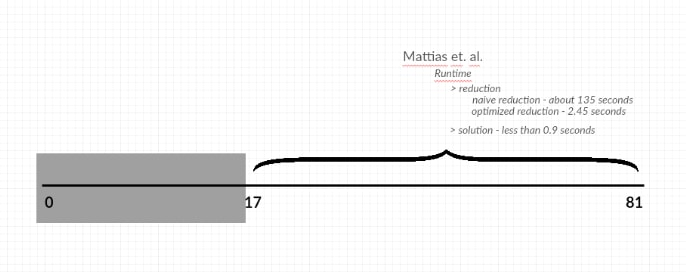
\includegraphics[width=0.9\textwidth]{framework.jpg}\label{fig:framework}}
  \caption{}
\end{figure}
\newpage

\section{Statement of the Problem}
This study intends to explore Sudoku puzzles not considered to be human-playable (below 17 clues) based on the reduction optimization by \cite{Harrysson} and also whether claim of \cite{Harrysson} that the difficulty in solving Sudoku in its Exact Cover equivalent is not based on the number of clues also applies to Sudoku puzzles not considered to be human-playable (below 17.

\section{Objectives of the Study}
The aim of this study is to continue the study of \cite{Harrysson} for the areas that were not explored, the Sudoku puzzles not considered to be human-playable (below 17 clues). Specifically:
\begin{enumerate}
\item As basis for comparison, to implement a usual brute force solution for Sudoku.
\item To solve Sudoku puzzles with less than 17 clues via reduction by:
\begin{enumerate}
\item Implementing Knuth$’$s DLX as described by \cite{Harrysson} in designing the reduction process.
\item Investigating result of DLX.
\begin{enumerate}
\item Interpreting the Exact Cover result as an instance of Sudoku
\end{enumerate}
\end{enumerate}
\item Compare the results of ? to the results of \cite{Harrysson}.
\item Verify if DLX can find all solutions of Sudoku within a considerable time limit.
\end{enumerate}

\section{Limitations}
This study will focus on continuing the study of \cite{Harrysson} but with the focus on exploring Sudoku puzzles not considered to be human-playable (below 17 clues); which were not explored in the study of \cite{Harrysson} At the same time, this study will focus mostly on solving 9$\times$9 Sudoku problems and not its other variants.

\section{Significance}
According to \cite{Harrysson}, the reduction process is arguable the most difficult since there is little written about the reduction is not much descriptive and that there is no significance in the number of clues in solving Sudoku in its Exact Cover equivalent. This study completes the study of \cite{Harrysson} by solving Sudoku puzzles not considered to be human-playable (below 17 clues). Also, to provide another description on how the reduction process  of Sudoku to its Exact Cover equivalent is done.

\chapter{Literature Review}
Many practical algorithms used for solving the Sudoku problems are fast enough to solve the puzzle but the solutions are not optimal. Thus, in solving the Sudoku problem, the optimal way of doing it would be through brute-force search and the most known algorithm for the brute-force search is backtracking \cite{Cazenave}. However, this solution is very slow and inefficient. \cite{Knuth} introduced a practically faster technique by applying a doubly-linked list to an algorithm he discovered, Algorithm X. The technique is called the Dancing Links (DLX). Knuth said that The Algorithm X and DLX, however, can only be applied to an Exact Cover Problem. As shown by \cite{Yato}, the Sudoku problem is NP-Complete by constructing an n\textsuperscript{2}$\times$n\textsuperscript{2} instance of Sudoku from an n$\times$n instance of a Latin Square Completion. Thus being an NP-Complete problem, the Sudoku problem is reducible to an Exact Cover problem, which is also an NP-Complete problem.\\

\cite{Berggren} compared three algorithms for solving the sudoku problem with the primary focus to measure and analyze the potential of these three algorithms in solving 17-clue Sudoku problems consisting of 49, 151 puzzles with a maximum solving time limit of 20 seconds. The algorithms were backtracking, rule-based and Boltzmann Machine. In addition, they also covered the difficulty rating of a sudoku puzzle, sudoku puzzle generation and how well the algorithms are fit for parallelizing. Out of the 49, 151 17-clue puzzles, the backtracking algorithm was not able to solve 1, 150 puzzles; 142 of those unsolved puzzles had unstable measurements. However, the algorithm was the second most efficient algorithm among the three tested algorithms. It had a mean solving time of 1.66 seconds for the solved puzzles. Given the maximum time limit 20 seconds to solve each puzzle, \cite{Berggren} suggests that if there had been more time, the other 1,150 unsolved puzzles would have been solved. However, the solving time for each puzzle may be different from each other and the solving times are unknown, it is impossible to know what their solving time is. Solving all 49, 151 17-clue puzzles with no unstable measurements, the Rule-based algorithm ended being the most efficient and accurate solving algorithm with a solving time of 0.02 seconds. With the use of logic rules with a polynomial time complexity, the thesis observed that there was a small time interval at which puzzles were solved. However, when the algorithm resolves to guessing, the time complexity is changed to exponential time thus the solving time will increase substantially - because, as noted, the guessing is simply like the backtracking algorithm. Using Boltzmann Machines proved to be very inefficient in solving the Sudoku problem. The algorithm was not able to solve all 49, 151 17-clue puzzles. Instead it needed at least 46 clues for it to be able to solve a puzzle. All results were still given a maximum solving time limit of 20 seconds. But the results turned out to be terrible and the measurements were unstable. In the end, as shown, only the backtracking algorithm and the rule-based algorithm were found to be capable of solving the sudoku problem.\\
	
	\cite{Harrysson} reduced 9$\times$9 human-playable Sudoku puzzles (17 or more clues) to an exact cover problem in the form of a matrix containing of only 1’s and 0’s. Each rule in sudoku is considered a constraint; thus, having four constraints: cell constraint, row constraint, column constraint and box constraint. The solution must cover all columns. Each cell in grid G has nine candidates which means that there must be nine rows in M for each cell where the first cell has 1’s in the first column for the first nine rows, the second cell has 1’s in the second column and so forth \cite{Harrysson}. Since there are 81 cells, there must be 81 columns for the cell constraint. And since each requires nine rows, M now therefore has 729 rows. At the same time, each constraint require 81 columns. Since there are four constraints, M would have a total of 324 columns. Hence, when reduced to an exact cover problem, a 9$\times$9 sudoku can be represented as a 729$\times$324 matrix of 1s and 0s. However, instead of using the original binary matrix, \cite{Harrysson} optimized its reduction by creating the links directly, thus reducing it directly to its Dancing Links form. This optimized reduction produced more efficient results than the naive reductions. The approximate runtime for the naive reductions was around 135 seconds while the approximate runtime for the optimized reductions was 2.54 seconds. \cite{Harrysson} only used Sudoku grids with 17 to 31 clues. As input, Harrysson and Laestander used all 49,151 17-clue Sudoku puzzles and gathered 14,236 Sudoku grids with clues from 18 to 31; majority of those grid having around 21 to 31 clues. Each grid timed from the start of the reduction to when a solution was found. Using the optimized reduction, results showed that the solving time of most Sudoku problems were solved in less than 0.5 seconds. All solutions, however, were solved in less than 0.9 seconds. In fact, most Sudoku grids were solved below 0.1 seconds. However, no experiment was made on finding all 6.67 $\times$ 10\textsuperscript{21} valid Sudoku solutions.\\
	
		The Pentomino puzzle is an example of an exact cover problem. Backtracking and depth-first traversal are examples of approaching the pentomino puzzle \cite{Nivasch}. As an example, Nivasch used an 8$\times$8 square with a 2$\times$2 hole in the middle and constructed a matrix with 72 columns - 60 for the cells on the board and 12 for the pentominoes. The first algorithm works by selecting the columns sequentially from the first 12 while the second algorithm works by selecting columns sequentially from the other 60. Nivasch implemented a program wherein an arbitrary 60-cell pattern is accepted as an input. The program then proceeds to build the matrix corresponding to the pattern being input, and applies the exact cover algorithm printing all the solutions it finds. The 8$\times$8 square mentioned above, found 520 solutions.\\
		
	The N Queens problem is another exact cover reducible problem \cite{Knuth}. There are many algorithms for solving the n-queens problem. This includes Genetic Algorithm (GA), Simulated Annealing (SA), Backtracking (BT), and Brute-force (BF) algorithms \cite{Mukherjee}. They proposed an algorithm which is the proposed genetic algorithm and the proposed simulated annealing using genetic algorithm and compared them together with brute-force and backtracking algorithms and found out that the Proposed Simulated Annealing using Genetic Algorithm takes less time than the Proposed Genetic Algorithm as it works on only one solution at a time and processes it to get the result but Proposed Genetic Algorithm gives better solution than the proposed Simulated Annealing using Genetic Algorithm as it works on a population of solutions and processes them to get the result. For Brute-force and backtracking, these algorithms can provide exact results but cannot provide solutions in ample time when the number of N is increased. Therefore, these two algorithms are not efficient to solve N-queens problem whereas the other two mentioned which is the proposed genetic algorithm and proposed simulated annealing using genetic algorithm provide good solutions to higher valued N.\\
	
	At the same time, in the field of computational music analysis, \cite{Bemman} reduced one of Milton Babbitt’s works, the Sheer Pluck, to an exact cover problem to find a sequence of distinct, non-overlapping aggregate regions that completely and exactly covers an irregular matrix of pitch class integers. The Sheer Pluck was constructed into a six-part all-partition array. The result of the array was a projection consisting of 6 rows and 696 pitch classes. The paper used a backtracking algorithm which yielded a sequence of 58 distinct partitions and aggregate-forming integer compositions that exactly cover the 696 class pitch integers.\\
	
While some of the above-mentioned papers have stated that the transformation from Sudoku to an Exact Cover is part of their paper, it is rather difficult to find a complete mapping of the Sudoku to exact cover, especially on Sudoku puzzles with clues. Further, while it was mentioned that the DLX implementation of Sudoku is much faster than the Brute Force in the exact cover equivalent, it is worth investigating the actual run time through our expirements.

\chapter{Theoretical Framework}
The computational complexity theory was the primary basis why the indirect solution of solving Sudoku using DLX is possible. According to computational complexity theory, computational problems are grouped together according to their inherent difficulty. Many complexity classes are defined using reduction. It is therefore worthy to discuss complexity classes in order to appreciate the reduction method.\\

This section is organized to contain the following theoretical foundations that are relevant in understanding reduction:
\begin{itemize}
  \item Complexity classes
  \vspace{-0.5cm}
  \item Reduction
\end{itemize}

\section{Complexity Classes}
There are about 70 known complexity classes \cite{Arora}. Probably the most studied classes P, NP, NP-Complete and NP-hard.\\

Nondeterministic Polynomial (NP) is a set of decision problems solvable in polynomial time by a theoretical non-deterministic Turing machine. Informally, it is a set of decision problems for which the instances where the answer is “yes” have efficiently verifiable proofs and these proofs have to be verifiable by a deterministic computation that can be performed in polynomial time. A language \emph{L} is in NP if and only if there exists a polynomial \emph{p} and \emph{q} deterministic Turing machine \emph{M}, such that:
\begin{enumerate}
\item For all \emph{x} and \emph{y}, the machine \emph{M} runs in time \emph{p}($\mid x \mid$) on input \emph{(x, y)},
\item For all \emph{x} in \emph{L}, there exists a string \emph{y} of length \emph{q($\mid x \mid$)} such that \emph{M(x, y) = 1},
\item For all \emph{x} not in \emph{L} and all strings \emph{y} of length \emph{q($\mid x \mid$)}, \emph{M(x, y) = 0}.
\end{enumerate}
On the other hand, Polynomial (P) is a generalization of NP. It contains all decision problems that can be solved by a deterministic Turing machine in polynomial time. Equivalently, it is the class of decision problems where each “yes” instance has a polynomial size certificate, and certificates can be checked by a polynomial time deterministic Turing machine. Cobham’s thesis says that P is the class of computational problems that are efficiently solved or tractable. Formally, a language \emph{L} is in P if and only if there exists a deterministic Turing machine \emph{M}, such that:
\begin{enumerate}
\item \emph{M} runs for polynomial time on all inputs,
\item for all \emph{x} in \emph{L}, \emph{M} outputs 1 and
\item for all \emph{x} not in \emph{L}, \emph{M} outputs 0.
\end{enumerate}
Furthermore, a decision problem \emph{C} is NP-complete if
\begin{enumerate}
\item \emph{C} is in NP,
\item Every problem in NP is reducible to \emph{C} in polynomial time, \emph{C} can be shown to be in NP by demonstrating that a candidate solution to C can be verified in polynomial time. The most notable characteristic of NP-complete problems is that no fast solution to them is known. The time required to solve the problem using any currently known algorithm increases very quickly as the size of the problem grows.
\end{enumerate}
Lastly, NP-Hard is a class of every problems where every problem \emph{L} in NP can be reducible in polynomial time to a certain problem \emph{H}; thus we can say \emph{H} is NP-Hard. For a certain NP-Complete to be considered a NP-Hard problem, there has to be a polynomial-time reduction from the NP-Complete problem to the NP-Hard problem. Basically, NP-Hard class of problems are as hard as the hardest problems in NP.\\
\begin{figure}[h]
  \centering
  {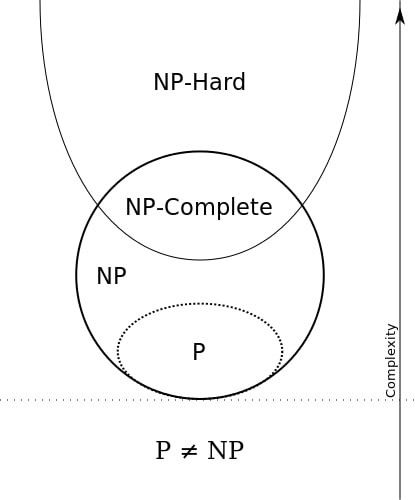
\includegraphics[width=0.4\textwidth]{venndiagram.jpg}\label{fig:venndiagram}}
  \caption{Venn Diagram for Class of Complexity Problems}
\end{figure}
\newpage
Sudoku problem and Exact Cover problems are known to be NP-Complete.\\

The decision question of the Sudoku problem is:
\begin{quote}
\textit{``Is there a solution such that there is no repeated digit in each row, column, and box?''}
\end{quote}

The decision question of the Exact Cover problem is:
\begin{quote}
\textit{``Is there a set of subsets such that the intersection of the subsets is empty and the union of the subsets is the set?''}
\end{quote}


\section{Exact Cover}
An exact cover is when each element in a given set X is contained in exactly one subset of X such that  the union of all subsets of a given set X covers the set X and the intersection of all subsets of the set X is empty. \\
Let S = \{A, B, C, D, E, F\} be a collection of subsets of a set X = \{1, 2, 3 ,4, 5, 6, 7\} such that:
\begin{center}
\begin{minipage}{0.5\linewidth}
\begin{itemize}
\item A = \{1, 4, 7\};
\vspace{-0.5cm}
\item B = \{1, 4\};
\vspace{-0.5cm}
\item C = \{4, 5, 7\};
\vspace{-0.5cm}
\item D = \{3, 5, 6\};
\vspace{-0.5cm}
\item E = \{2, 3, 6, 7\}; and
\vspace{-0.5cm}
\item F = \{2, 7\}\\
\end{itemize}
\end{minipage}
\end{center}
\newpage
\noindent Alternatively, the above S can also be represented as a binary matrix as below\\
\begin{center}
\begin{tabular}{ m{0.5cm}  m{0.5cm} m{0.5cm} m{0.5cm} m{0.5cm} m{0.5cm} m{0.5cm} m{0.5cm}} 
& \textbf{1} & \textbf{2} & \textbf{3} & \textbf{4} & \textbf{5} & \textbf{6} & \textbf{7}\\ 
\textbf{A} & 1 & 0 & 0 & 1 & 0 & 0 & 1\\ 
\textbf{B} & \textbf{1} & 0 & 0 & \textbf{1} & 0 & 0 & 1\\ 
\textbf{C} & 0 & 0 & 0 & 1 & 1 & 0 & 1\\
\textbf{D} & 0 & 0 & \textbf{1} & 0 & \textbf{1} & \textbf{1} & 0\\
\textbf{E} & 0 & 1 & 1 & 0 & 0 & 1 & 1\\
\textbf{F} & 0 & \textbf{1} & 0 & 0 & 0 & 0 & \textbf{1}\\
\end{tabular}
\end{center}
\vspace{0.8cm}
Then the subcollection S* = \{B, D, F\} is an exact cover since:
\begin{center}
\begin{minipage}{0.5\linewidth}
\begin{itemize}
\item B $\cup$ D $\cup$ F = X; and
\vspace{-0.5cm}
\item B $\cap$ D $\cap$ F = {\O}\\
\end{itemize}
\end{minipage}
\end{center}
Formally, given a collection S of subsets of X, an exact cover of X is the subcollection S* of S that satisfies the following conditions:
\begin{enumerate}[label=\alph*.]
\item The intersection of any two distinct subsets in S* is empty (the subsets in S* are pairwise disjoint)
\item The union of the subsets in S* is X.
\end{enumerate}


\section{Reduction}
NP-complete problems are studied because the ability to quickly verify solutions to a problem (NP) seems to correlate with the ability to quickly solve that problem (P). It is not known whether every problem in NP can be quickly solved—this is called the P versus NP problem. But if \textit{any NP-complete problem} can be solved quickly, then \textit{every problem in NP} can, because the definition of an NP-complete problem states that every problem in NP must be quickly reducible to every NP-complete problem (that is, it can be reduced in polynomial time). Because of this, it is often said that NP-complete problems are \textit{every problem in NP} or \textit{more difficult} than NP problems in general.\\

Since any NP-complete problem can be reduced to another NP-Complete problem, its solution can be derived indirectly using reduction.\\

Reduction is an algorithm transforming one problem into another problem such that, under N. If a language A $\subseteq$ \{0, 1\}* is polynomial-time Karp reducible to a language B $\subseteq$ \{0, 1\}* denoted by A $\leq$ p B if there is a polynomial-time computable function 
f : \{0, 1\}* $\rightarrow$ \{0, 1\}* such that for every x $\in$ \{0, 1\}*, x $\in$ A if and only if f(x) $\in$ B.

\begin{figure}
  \centering
  {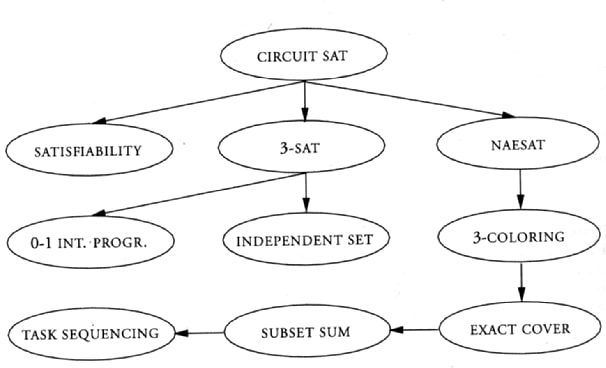
\includegraphics[width=0.7\textwidth]{circuitsat.jpg}}
  \caption{Reduction of CircuitSat Problem to other known NP problems}
\end{figure}
The figure above illustrates the reduction of other CircuitSat Problem to other known NP problems. The reduction of CircuitSat to 3-Sat has led to the growth of the number of problems belonging to NP-Complete class.\\

\noindent In this study, the reduction of Sudoku to Exact Cover will have two implications:
\begin{itemize}
\item That the solution of Sudoku in can be solved through the terms of Exact Cover.
\item That the theoretical runtime of solving through exact cover is still the within the same class.
\end{itemize}

\chapter{Methodology}
The brute force method will be used as the basis of comparison of the other solutions. Such that the Methodology is organized as follows:
\begin{enumerate}
\item Brute-force Implementation
\vspace{-0.5cm}
\item Reduction of Sudoku to Exact Cover
\vspace{-0.5cm}
\item Solving the Exact Cover (through Algorithm X and DLX)
\end{enumerate}
Lastly, the Sudoku puzzles will be classified so that the algorithms’ performance can be observed.\\

For uniform notation, the following is defined:
\begin{itemize}
\item Each row in the Sudoku grid will be denoted as \textit{r}.
\item Each column in the Sudoku grid will be denoted as \textit{c}.
\item Each value in a cell in the Sudoku grid will be denoted as \textit{n}.
\item The Sudoku puzzle will be denoted as \textit{P}.
\item All possibilities or combinations in the Sudoku puzzle is denoted as a three-tuple {\itshape P\textsubscript{i} = \{\ r, c, n \}}.
\item The Exact Cover X will be a four-tuple {\itshape X\textsubscript{j} = \{\ cellCons, rowCons, colCons, boxCons\}} such that it is the st of given clues in a Sudoku problem.
\end{itemize}

\section{Brute-force Implementation}
Analyzing the results of the Brute-force implementation for Sudoku will show the difference in efficiency in solving the Sudoku problem. Generally, when using the Brute-force algorithm in solving any problem, one has to implement its four main procedures: \emph{first}, \emph{next}, \emph{valid}, and \emph{output}. These procedures should take a data P as a parameter for the particular instance of the problem to be solved. The procedures are also defined as the following:
\begin{enumerate}
\item first (\emph{P}): generate a first candidate solution for \emph{P}.
\item next (\emph{P}, \emph{n}): generate the next candidate \emph{P} after the current one \emph{n}.
\item valid (\emph{P}, \emph{n}): check whether candidate \emph{n} is a solution for \emph{P}.
\item output (\emph{P}, \emph{n}): use the solution \emph{n} of \emph{P} as appropriate to the application.
\end{enumerate}
The \emph{first} procedure should return \emph{null} if there are no candidates of the instance \emph{P}. The \emph{next} procedure must also tell that when there are no more candidates for the instance \emph{P}, after the current one \emph{n}. The Brute-force algorithm is the expressed as\\

\begin{algorithm}
\caption{Brute-force Algorithm}\label{bruteforce}
\begin{algorithmic}[1]
\State $n\gets first(P)$
\While{$n\not=null$}
\If{\textit{valid(P, n)}}
\textit{output(P, n)}
\EndIf
\State $n\gets (P, n)$
\EndWhile\label{bruteforceendwhile}
\State \textbf{end while}
\end{algorithmic}
\end{algorithm}

In implementing  the Brute-force algorithm in the Sudoku problem, the algorithm will visit empty cells in some order defined by the programmer. When visiting each cell, the algorithm fills in digits in sequence of available choices and backtracks once a dead-end is reached. For every backtrack, the algorithm iterates the digit in the cell most recently filled before the the cell where the dead end was seen. If all possible digits are already tried by the algorithm, the algorithm again does a backtrack and repeats the same process until a solution is found. The algorithm of the backtracking will be as follows:\\

\begin{algorithm}
\caption{Backtracking Algorithm}\label{backtracking}
\begin{algorithmic}[1]
\newcommand\NoDo{\renewcommand\algorithmicdo{}}
\If{\textit{choices(empty)}}
\textit{true}
\EndIf
\For{1 $\rightarrow$ 9}
\State \textbf{try} \textit{choice n}
\If{\textit{solved(n)}} \textit{true}
\EndIf
\State \textbf{unmake} \textit{choice n}
\EndFor
\State \textbf{return} $false$
\end{algorithmic}
\end{algorithm}

\begin{figure}[h]
  \centering
  \stackunder[2pt]{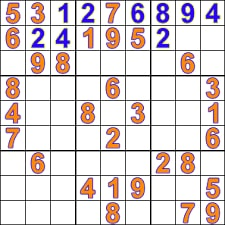
\includegraphics[width=0.4\textwidth]{bruteforcesudoku.jpg}}{\footnotesize{Brute-force: orange digits are fixed while blue ones are partial solutions}}
\end{figure}

\section{Reduction of Blank Sudoku to Exact Cover}
Finding a more efficient way of solving the Sudoku problem is one of the main focuses of this paper, the next step will be the implementing of the reduction of the Sudoku problem to an exact cover problem. In the standard 9$\times$9 Sudoku variant, in which each of 9$\times$9 cells is assigned one of 9 numbers, there are 9$\times$9$\times$9=729 possibilities. Using obvious notation for rows, columns and numbers, the possibilities can be labeled R\textsubscript{1}C\textsubscript{1}\textbf{\#1}, R\textsubscript{1}C\textsubscript{1}\textbf{\#2}, ..., R\textsubscript{9}C\textsubscript{9}\textbf{\#9} (Harryson and Laestander, 2014). (Harryson and Laestander, 2014) provides detail in reducing the Sudoku problem to an exact cover problem containing four constraints:
\begin{enumerate}[label=\alph*.]
\item cell constraint
\vspace{-0.5cm}
\item row constraint
\vspace{-0.5cm}
\item column constraint
\vspace{-0.5cm}
\item box constraint
\end{enumerate}
The fact that each kind of constraint involves exactly one of something is what makes Sudoku an exact hitting set problem. The constraints can be represented by constraint sets. The problem is to select possibilities such that each constraint set contains (i.e., is hit by) exactly one selected possibility. \cite{Harrysson} uses the following convention for Cell Constraint rows, Row Constraint rows, Column Constraint rows, and Box Constraint rows.\\

\noindent To avoid confusion in the format, the matrix will be arranged as cell constraint, row constraint, column constraint, and then box constraint. Such that the first 81 columns of the matrix will belong to the cell constraint and the next 81 columns will belong to the row constraint as is shown in the representation below.\\

\noindent The following possibilities in the Sudoku Grid should be transformed to its Exact Cover form as shown below:\\
{\itshape P\textsubscript{i} = \{\ 1, 1, 1 \} $\Rightarrow$ X\textsubscript{j} = \{\ 1, 82, 163, 244 \}}\\
{\itshape P\textsubscript{i} = \{\ 1, 1, 2 \} $\Rightarrow$ X\textsubscript{j} = \{\ 1, 83, 164, 245 \}}\\
...\\
{\itshape P\textsubscript{i} = \{\ 1, 1, 1 \} $\Rightarrow$ X\textsubscript{j} = \{\ 81, 162, 243, 324 \}}\\
\newline
Or as shown in the illustration below:
\begin{center}
\begin{tabular}{m{0.2cm} m{2.5cm} m{2.9cm} m{3cm} m{3cm} m{2.5cm}}
& & & \textbf{Constraints} & &
\end{tabular}
\end{center} 
\begin{tabular}{m{2.5cm} m{3cm} m{3cm} m{3cm} m{3cm}}
{\itshape P\textsubscript{i} = \{\ r, c, n \}} & \textbf{cell} & \textbf{row} & \textbf{column} & \textbf{box}\\ 
& \textbf{1\hspace{0.5cm} 2\hspace{0.5cm} ... \hspace{0.1cm}	81} & \textbf{82\hspace{0.2cm} 83\hspace{0.2cm} ... \hspace{0.3cm}	162} & \textbf{163\hspace{0.2cm} 164\hspace{0.1cm} ... \hspace{0.1cm}	243} & \textbf{244\hspace{0.2cm} 245\hspace{0.1cm} ... \hspace{0.3cm}	324}\\ 
{\itshape P\textsubscript{i} = \{\ 1, 1, 1 \}} & 1\hspace{0.5cm} 0\hspace{0.5cm} ... \hspace{0.2cm} 0 & 1\hspace{0.5cm} 0\hspace{0.3cm} ... \hspace{0.5cm} 0 & 1\hspace{0.7cm} 0\hspace{0.5cm} ... \hspace{0.3cm} 0 & 1\hspace{0.7cm} 0\hspace{0.5cm} ... \hspace{0.3cm} 0\\ 
{\itshape P\textsubscript{i} = \{\ 1, 1, 2 \}} & 1\hspace{0.5cm} 0\hspace{0.5cm} ... \hspace{0.2cm} 0 & 0\hspace{0.5cm} 1\hspace{0.3cm} ... \hspace{0.5cm} 0 & 0\hspace{0.7cm} 1\hspace{0.5cm} ... \hspace{0.3cm} 0 & 0\hspace{0.7cm} 1\hspace{0.5cm} ... \hspace{0.3cm} 0\\ 
\hspace{0.7cm}... & &\hspace{2cm} ... & & \\
{\itshape P\textsubscript{i} = \{\ 9, 9, 9 \}} & 0\hspace{0.5cm} 0\hspace{0.5cm} ... \hspace{0.2cm} 1 & 0\hspace{0.5cm} 0\hspace{0.3cm} ... \hspace{0.5cm} 1 & 0\hspace{0.7cm} 0\hspace{0.5cm} ... \hspace{0.3cm} 1 & 0\hspace{0.7cm} 0\hspace{0.5cm} ... \hspace{0.3cm} 1\\ 
\end{tabular}
\newline
\newline

\textbf{Cell Constraint:} Each cell in the Sudoku Grid has nine candidates which means that there must be nine rows in the Exact Cover Matrix for each cell where the first cell has 1’s in the first column for the first nine rows, the second cell has 1’s in the second column and so forth.  For example, the constraint set for row 1 and column 1, which can be labeled r1c1, contains the 9 possibilities for row 1 and column 1 but different numbers.\\
r\textsubscript{1}c\textsubscript{1} = \{r\textsubscript{1}c\textsubscript{1}\textbf{\#1}, r\textsubscript{1}c\textsubscript{1}\textbf{\#2}, r\textsubscript{1}c\textsubscript{1}\textbf{\#3}, r\textsubscript{1}c\textsubscript{1}\textbf{\#4}, r\textsubscript{1}c\textsubscript{1}\textbf{\#5}, r\textsubscript{1}c\textsubscript{1}\textbf{\#6}, r\textsubscript{1}c\textsubscript{1}\textbf{\#7}, r\textsubscript{1}c\textsubscript{1}\textbf{\#8}, r\textsubscript{1}c\textsubscript{1}\textbf{\#9}\}.\\

\textbf{Row Constraint:} In each cell of the row constraint, the 1’s are placed in a new column for each row of the nine rows in the Exact Cover Matrix. The same pattern is applied for the first nine cells in the Sudoku Grid - first 81 rows in the Exact Cover Matrix. The next row constraint starts at the 10th cell of the Sudoku Grid or at the 82nd row of the Exact Cover Matrix. And the next constraint starts at the 19th cell or at the 163rd row and so on and so forth.\\
For example, the constraint set for all columns of row 1 having the value 1, which can be labeled r1 \textbf{\#1}, contains the 9 possibilities for row 1 and number 1 but different columns:\\
r\textsubscript{1}\textbf{\#1} = \{r\textsubscript{1}c\textsubscript{1}\textbf{\#1}, r\textsubscript{1}c\textsubscript{2}\textbf{\#1}, r\textsubscript{1}c\textsubscript{3}\textbf{\#1}, r\textsubscript{1}c\textsubscript{4}\textbf{\#1}, r\textsubscript{1}c\textsubscript{5}\textbf{\#1}, r\textsubscript{1}c\textsubscript{6}\textbf{\#1}, r\textsubscript{1}c\textsubscript{7}\textbf{\#1}, r\textsubscript{1}c\textsubscript{8}\textbf{\#1}, r\textsubscript{1}c\textsubscript{9}\textbf{\#1}\}.\\

\textbf{Column Constraint:} The pattern in the column constraint looks similar to the row constraint pattern where the 1’s are placed in a new column for the first nine rows in the Exact Cover Matrix. This goes on until the ninth cell. However, unlike the row constraint, the next column constraint starts 1 cell forward from where the last column constraint ended.\\

For example, the constraint set for all rows in column 1 having the value 1, labeled c1 \textbf{\#1}, contains the 9 possibilities for column 1 and number 1 but different rows:\\
c\textsubscript{1}\textbf{\#1} = \{r\textsubscript{1}c\textsubscript{1}\textbf{\#1}, r\textsubscript{2}c\textsubscript{1}\textbf{\#1}, r\textsubscript{3}c\textsubscript{1}\textbf{\#1}, r\textsubscript{4}c\textsubscript{1}\textbf{\#1}, r\textsubscript{5}c\textsubscript{1}\textbf{\#1}, r\textsubscript{6}c\textsubscript{1}\textbf{\#1}, r\textsubscript{7}c\textsubscript{1}\textbf{\#1}, r\textsubscript{8}c\textsubscript{1}\textbf{\#1}, r\textsubscript{9}c\textsubscript{1}\textbf{\#1}\}.\\

\textbf{Box Constraint:} Unlike the previous constraints, the box constraint would seem to an irregular pattern at first. For the constraint of three complete boxes, if they are in the same box in the Sudoku Grid, their columns are equal in the Exact Cover Matrix. Since each box has similar rules with the row and column, that each box must only have unique integer from one to nine, in each cell in the Sudoku Grid the columns placed just like the row constraint in the Exact Cover Matrix and continues until the next cell. For example, the constraint set for box 1 (top-most left-most box) having the value 1 in each cell, which can be labeled B1 \textbf{\#1}, contains the 9 possibilities for the cells in box 1 and number 1:\\
B\textsubscript{1}\textbf{\#1} = \{r\textsubscript{1}c\textsubscript{1}\textbf{\#1}, r\textsubscript{1}c\textsubscript{2}\textbf{\#1}, r\textsubscript{1}c\textsubscript{3}\textbf{\#1}, r\textsubscript{2}c\textsubscript{1}\textbf{\#1}, r\textsubscript{2}c\textsubscript{2}\textbf{\#1}, r\textsubscript{2}c\textsubscript{3}\textbf{\#1}, r\textsubscript{3}c\textsubscript{1}\textbf{\#1}, r\textsubscript{3}c\textsubscript{2}\textbf{\#1}, r\textsubscript{3}c\textsubscript{3}\textbf{\#1}\}.\\

Since there are 9 rows, 9 columns, 9 boxes and 9 numbers, there are 9$\times$9=81 row-column constraint sets, 9$\times$9=81 row-number constraint sets, 9$\times$9=81 column-number constraint sets, and 9$\times$9=81 box-number constraint sets: 81+81+81+81=324 constraint sets in all.\\

The end result of the reduction is a binary matrix, the exact cover instance of the Sudoku.\\

Since in a 9$\times$9 Sudoku there are 81 cells and each cell has nine possible values ranging from 1 to 9, nine rows for each cell would be required of the matrix. Thus, we would be having a total of 729 rows in the matrix. At the same time, each constraint requires 81 columns each. Since there are four constraints, there would be a total of 324 columns in the matrix. Therefore, we would be having a 729$\times$324 binary matrix. To generate the Exact Cover matrix, an algorithm based on the four constraints will be formulated.\\

The matrix will then be evaluated using two methods: The naive implementation of Algorithm X and the implementation of Algorithm X with the use of Dancing Links technique. The results of  these two reduction methods will also compared to each other after implementation.

\subsection{Reduction of Sudoku with Clues to Exact Cover}
Several methods are employed for reducing sudoku with clues. When a clue is provided, that clue is already chosen to be part of the solution. Other configuration of that clue are deemed useless. Some mechanisms to deal this include:
\begin{enumerate}
\item Exclusion of the excluded rows
\vspace{-0.3cm}
\item Setting one or more of the four 1’s into zero
\vspace{-0.3cm}
\item Setting all values of the row into zero
\end{enumerate}

The option one is the optimal choice since it will significantly reduce the size of the matrix, and improve the performance of the computation because these rows are not explored. However,  need to still include the rows in order to have a uniform matrix size in all kinds of matrix in our samples. In this case, we use the option 3 above.\\

The position of 1’s in each selected row from the exact cover matrix will define the position of solution in the Sudoku grid. For example, for {\itshape P\textsubscript{i} = \{\ 5, 5, 7 \}} in the puzzle below, its representation in the matrix is shown as  in the figure below.
\begin{table}[!ht]
\begin{tabular}{m{2.5cm} m{3cm} m{3cm} m{3cm} m{3cm}}
{\itshape P\textsubscript{i} = \{\ r, c, n \}} & \textbf{cell} & \textbf{row} & \textbf{column} & \textbf{box}\\ 
& \textbf{1\hspace{0.1cm}...\hspace{0.1cm} 41 \hspace{0.1cm}... \hspace{0.1cm}	81} & \textbf{82\hspace{0.1cm} ... 124 \hspace{0.1cm}... 162} & \textbf{163 ... 205 ... 243} & \textbf{244 ... 286 ... 324}\\ 
{\itshape P\textsubscript{i} = \{\ 5, 5, 7 \}} & 0\hspace{0.1cm} ...\hspace{0.1cm} 1 \hspace{0.2cm}... \hspace{0.1cm}	0 & 0 \hspace{0.2cm} ...\hspace{0.2cm} 1 \hspace{0.3cm}... \hspace{0.1cm}	0 & 0\hspace{0.4cm} ...\hspace{0.2cm} 1\hspace{0.28cm}... \hspace{0.1cm}0 & 0\hspace{0.4cm} ...\hspace{0.2cm} 1 \hspace{0.18cm}... \hspace{0.1cm}	0\\ 
\end{tabular}
\caption{{Exact cover representation of {\itshape P = \{\ 5, 5, 7 \}}}}
\end{table}

\begin{figure}[h]
\begin{minipage}{0.5\textwidth}
{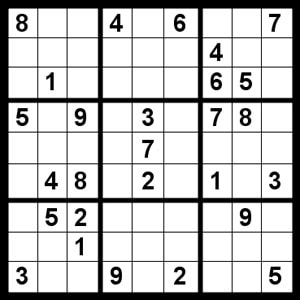
\includegraphics[width=0.7\textwidth]{sampleduko.jpg}}
\newline
\end{minipage}
\hspace*{-1cm}$\Rightarrow$\hspace{1cm}
\begin{minipage}{0.5\textwidth}
0001...0001000...00001000...001\\
0000...0000000...00000000...000\\
0000...0000000...00000000...000\\
0000...0000000...00000000...000\\
....\\
0100...0001000...00000010...001\\
0000...0000000...00000000...000\\
0000...0000000...00000000...000\\
0000...0000000...00000000...000\\
\end{minipage}
\caption{Sudoku Problem and its Exact Cover equivalent}
\end{figure}

\newpage
\section{Exact Cover Algorithms}
After using the Brute-force search in solving Sudoku problems, the Sudoku problems will then be solved in its Exact Cover equivalent form. Exact Cover algorithms will be used in solving the problems. Knuth describes Algorithm X as the most obvious trial-and-error approach in \cite{Knuth}. It is a recursive backtracking algorithm that is generally useful in solving exact cover problems. Theoretically, the average search time complexity of Algorithm X is O(n). Another algorithm for solving exact cover problems is the Dancing Links. Dancing Links is the technique used by Donald Knuth to efficiently implement Algorithm X. The naive implementation of Algorithm X was observed by Knuth to take up an excessive amount of time in searching for 1’s. To solve this problem, Knuth used a sparse matrix where only 1’s are stored, thus, improving the complexity from O(n) to O(1).

\subsection{Algorithm X Implementation}
Algorithm X will be implemented first, once the reduction is complete, as it  stands as a basis for comparison among both methods used in solving the exact cover problem of a Sudoku. This is tested whether it provides a more efficient solution to solving the problem or not. Algorithm X is as follows:
\begin{enumerate}
\item If the matrix A has no columns, the current partial solution is a valid solution; terminate immediately.
\vspace{-0.5cm}
\item Otherwise, choose a column \emph{c} deterministically.
\vspace{-0.5cm}
\item Choose a row \emph{r} such that A\textsubscript{r1c}  = 1 nondeterministically.
\vspace{-0.5cm}
\item Include row \emph{r} in the partial solution.
\vspace{-0.5cm}
\item For each column \emph{j} such that A\textsubscript{r1j}  = 1,
\vspace{-0.5cm}
\begin{enumerate}
\item For each row \emph{i} A\textsubscript{r1j}  = 1,
\vspace{-0.5cm}
\begin{enumerate}
\item Delete row \emph{i} from matrix \emph{A}.
\vspace{-0.5cm}
\end{enumerate}
\item Delete column \emph{j} from matrix \emph{A}.
\vspace{-0.5cm}
\end{enumerate}
\item Repeat this algorithm recursively on the reduced matrix \emph{A}.
\end{enumerate}

\subsection{DLX Implementation}
After using Algorithm X to solve the Sudoku problem, this paper then proceeds to its most important implementation, using the Dancing Links(DLX) technique on Algorithm X in order to solve the Sudoku problem. The Dancing Links is a technique suggested by Donald Knuth to solve an exact cover problem using Algorithm X more efficiently. DLX concept is simply unlinking two connected nodes and also potentially link back again those two nodes. The idea of DLX is based on the observation that in a circular doubly linked list of nodes,\\
$L[R[x]] \leftarrow L[x];\\
R[L[x]] \leftarrow R[x];$\\
will remove node x from the list, while\\
$L[R[x]] \leftarrow x;\\
R[L[x]] \leftarrow x;$\\
will restore x’s position in the list, assuming that x.left and x.right have been left unmodified.
\begin{center}
\begin{tabular}{ m{0.5cm}  m{0.5cm} m{0.5cm} m{0.5cm} m{0.5cm} m{0.5cm} m{0.5cm} m{0.5cm}} 
& \textbf{1} & \textbf{2} & \textbf{3} & \textbf{4} & \textbf{5} & \textbf{6} & \textbf{7}\\ 
\textbf{A} & 0 & 0 & 1 & 0 & 1 & 1 & 0\\ 
\textbf{B} & 1 & 0 & 0 & \textcolor{red}{1} & 0 & 0 & \textcolor{red}{1}\\ 
\textbf{C} & 0 & 1 & 1 & 0 & 0 & 1 & 0\\
\textbf{D} & 1 & 0 & 0 & \textcolor{red}{1} & 0 & 0 & 0\\
\textbf{E} & 0 & 1 & 0 & 0 & 0 & 0 & 1\\
\textbf{F} & 0 & 0 & 0 & 1 & 1 & 0 & 1\\
\end{tabular}
\end{center}

The above instance is implemented as linked list below. The DLX follows algorithm X as described in \textit{Algorithm 2}.  However, links are employed instead of a matrix. To delete column A (as in step 5.b of Algorithm X), the link from Header to A is re-assigned to B and the link from B to A is reassigned to Header as shown in the following figure. This is also the case to the nodes when removing rows (in step 5.a.i)
\begin{figure}[h]
  \centering
  {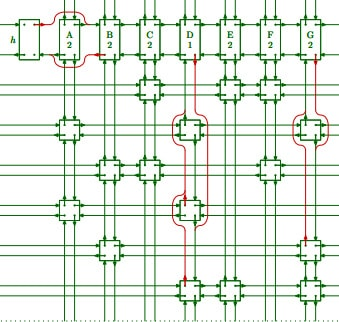
\includegraphics[width=0.3\textwidth]{dlxlinkedlist.jpg}\label{fig:linkedlist}}
\end{figure}
\newline
The links are restored using the second set of equations.

\section{Interpretation of Exact Cover result}
The position of 1’s in each selected row from the exact cover matrix will define the position of solution in the Sudoku grid. For example, for {\itshape X\textsubscript{j} = \{\ 6, 89, 215, 260 \}} as shown in its representation in the matrix, its equivalent Sudoku instance is {\itshape P\textsubscript{i} = \{\ 1, 6, 8 \}} as shown in the Sudoku puzzle below.

\begin{table}[!ht]
\begin{tabular}{m{1cm} m{3cm} m{3cm} m{3cm} m{3cm}}
& \textbf{cell} & \textbf{row} & \textbf{column} & \textbf{box}\\ 
& \textbf{1\hspace{0.1cm}...\hspace{0.1cm} 6 \hspace{0.1cm}... \hspace{0.1cm}	81} & \textbf{82\hspace{0.1cm} ... 89 \hspace{0.1cm}... 162} & \textbf{163 ... 215 ... 243} & \textbf{244 ... 260 ... 324}\\ 
& 0 ...\hspace{0.1cm} 1 \hspace{0.1cm}... \hspace{0.1cm}	0 & 0 \hspace{0.2cm} ...\hspace{0.1cm} 1 \hspace{0.2cm}... \hspace{0.1cm}	0 & 0\hspace{0.4cm} ...\hspace{0.2cm} 1\hspace{0.28cm}... \hspace{0.1cm}0 & 0\hspace{0.4cm} ...\hspace{0.2cm} 1 \hspace{0.18cm}... \hspace{0.1cm}	0\\ 
\end{tabular}
\caption{{\itshape X\textsubscript{j} = \{\ 6, 89, 215, 260 \}}}
\end{table}

\begin{figure}[h]
  \centering
  {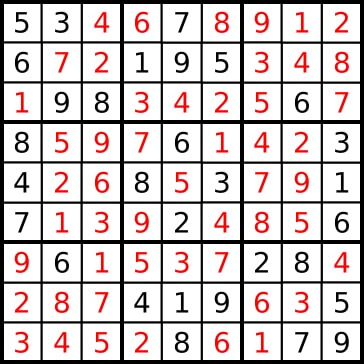
\includegraphics[width=0.3\textwidth]{Sudoku_Puzzle_Answer.jpg}\label{fig:puzzleanswer}}
  \caption{Completed Sudoku Puzzle}
\end{figure}

\section{Sudoku Puzzles}
\begin{figure}[h]
  \centering
  {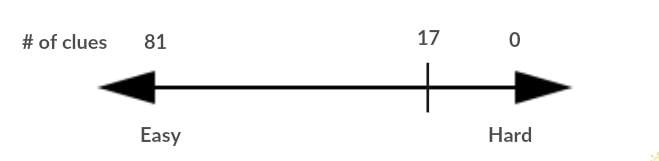
\includegraphics[width=0.7\textwidth]{clues.jpg}\label{fig:clues}}
\end{figure}
In solving a Sudoku puzzle, the higher the number of clues, the easier it would be solve the problem. The least known number of clues in order to have a unique solution in for a Sudoku problem is 17 \cite{Jones}. \cite{McGuire} also made a research that there are no 16-clue Sudoku puzzles. A Sudoku puzzle with less than 17 clues would have the tendency to produce more than one output. Thus, it would invalid the puzzle from being a Sudoku puzzle.\\

This paper will investigate the following sudoku puzzles:
\begin{enumerate}
\item Blank (zero-clue) sudoku
\item 1-16 clue puzzles (with several solutions)
\item 17-clue puzzles (each has single solution)
\item 18-25 clue sudoku (considered as easy puzzles)\\
\end{enumerate}
\newpage
\begin{figure}[h]
  \centering
  \subfloat[Blank Sudoku]{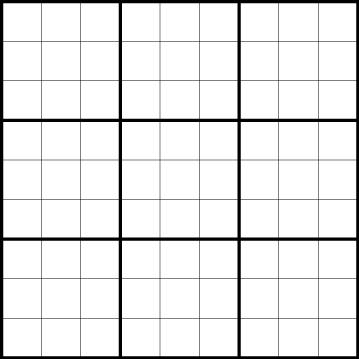
\includegraphics[width=0.4\textwidth]{blanksudoku.jpg}\label{fig:blanksudoku}}
  \hspace{2cm}
  \vspace{3cm}
  \subfloat[16-clue Sudoku]{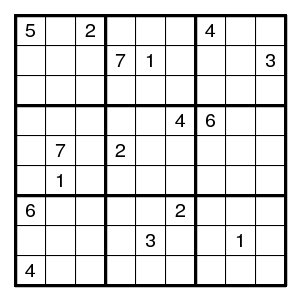
\includegraphics[width=0.4\textwidth]{16-clue.jpg}\label{fig:16-clue}}
  \hfill
  \subfloat[17-clue Sudoku]{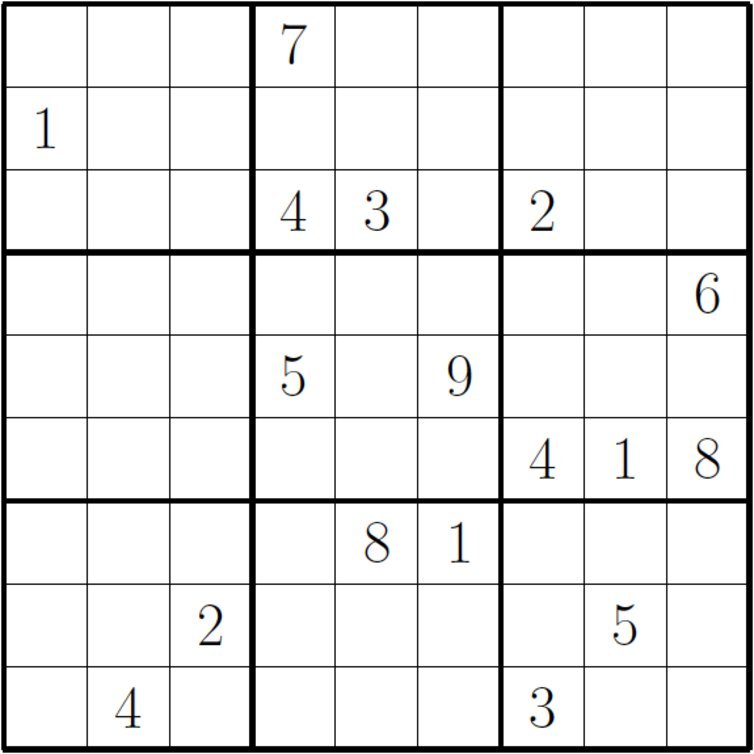
\includegraphics[width=0.4\textwidth]{17-clue.jpg}\label{fig:17-clue}}
  \hspace{2cm}
  \subfloat[25-clue Sudoku]{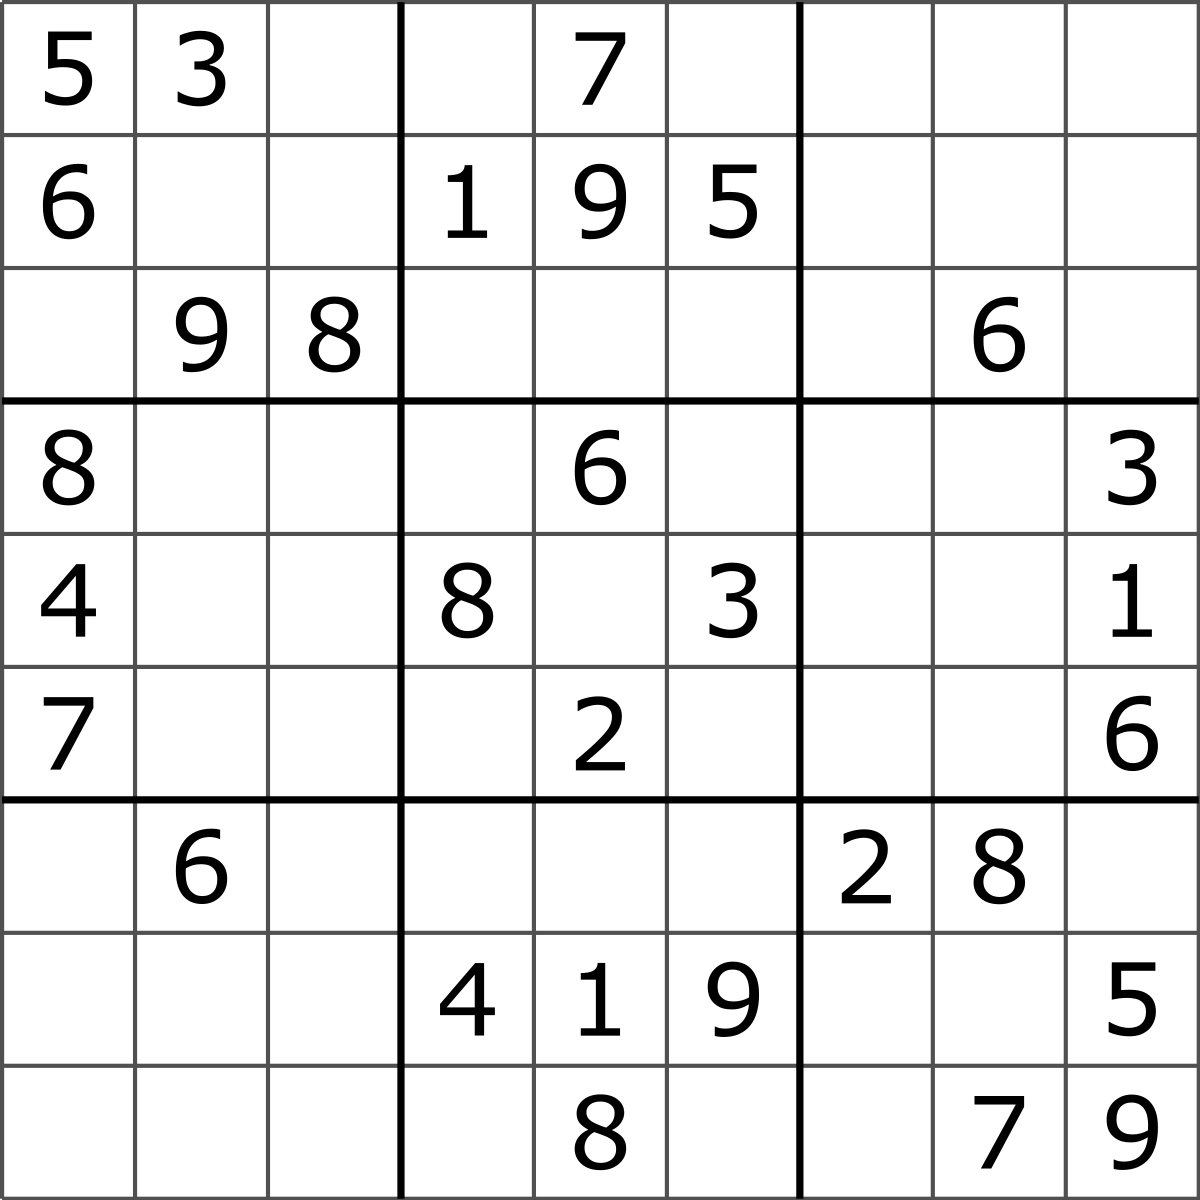
\includegraphics[width=0.4\textwidth]{25-clue.jpg}\label{fig:25-clue}}
  \caption{Classifications of Sudoku Puzzles}
\end{figure}
\noindent For each test, 3 to 5 runs will be done and the average runtime will be noted.

\newpage
\begin{center}
\LARGE \hspace{2.5cm} \textbf{Research Schedule}
\newline
\end{center}

The table below shows the list of activities and the corresponding time frame for this study.
\begin{table}[!ht]
\begin{center}
\begin{tabular}{p{3.75in} | p{2in}}
\hline
&\\
\textbf{Activities} & \textbf{Date / Period}\\
&\\
\hline
\hline
&\\
Implementation of the design of the reduction process from Sudoku to Exact Cover & June 2017 to July 2017\\
&\\
\hline
&\\
Implementation of the Algorithm X and Dancing Links, Experimentation, and Research Report writing & July 2017 to Middle of August 2017\\
&\\
\hline
&\\
Final Research Presentation & Late August 2017\\
&\\
\hline
&\\
Revision and Finalization & Late August 2017 to Early September 2017\\
&\\
\hline
&\\
Bookbinding and Submission of Copies & Middle of September 2017\\
&\\
\hline
\end{tabular}
\end{center}
\caption{Research Schedule from June 2017 to September 2017}
\end{table}

\addcontentsline{toc}{chapter}{References}
\nocite{*}
\bibliography{references}

\end{document}\grid
